\subsection{Gebruikerbestuur, intekening en registrasie onderdeel}

Die gebruikerbestuur, intekening en registrasie onderdeel is 'n kritieke
komponent van die toepassing, aangesien dit die gebruikers se
toegang tot die stelsel beheer. Dit sluit die bestuur van gebruikersprofiele,
intekening, registrasie, en die hantering van gebruikersrolle in. Hierdie
onderdeel is verantwoordelik vir die verifikasie van gebruikers, die hantering
van gebruikerssessies, en die bestuur van gebruikersdata.

\begin{figure}[ht]
    \centering
    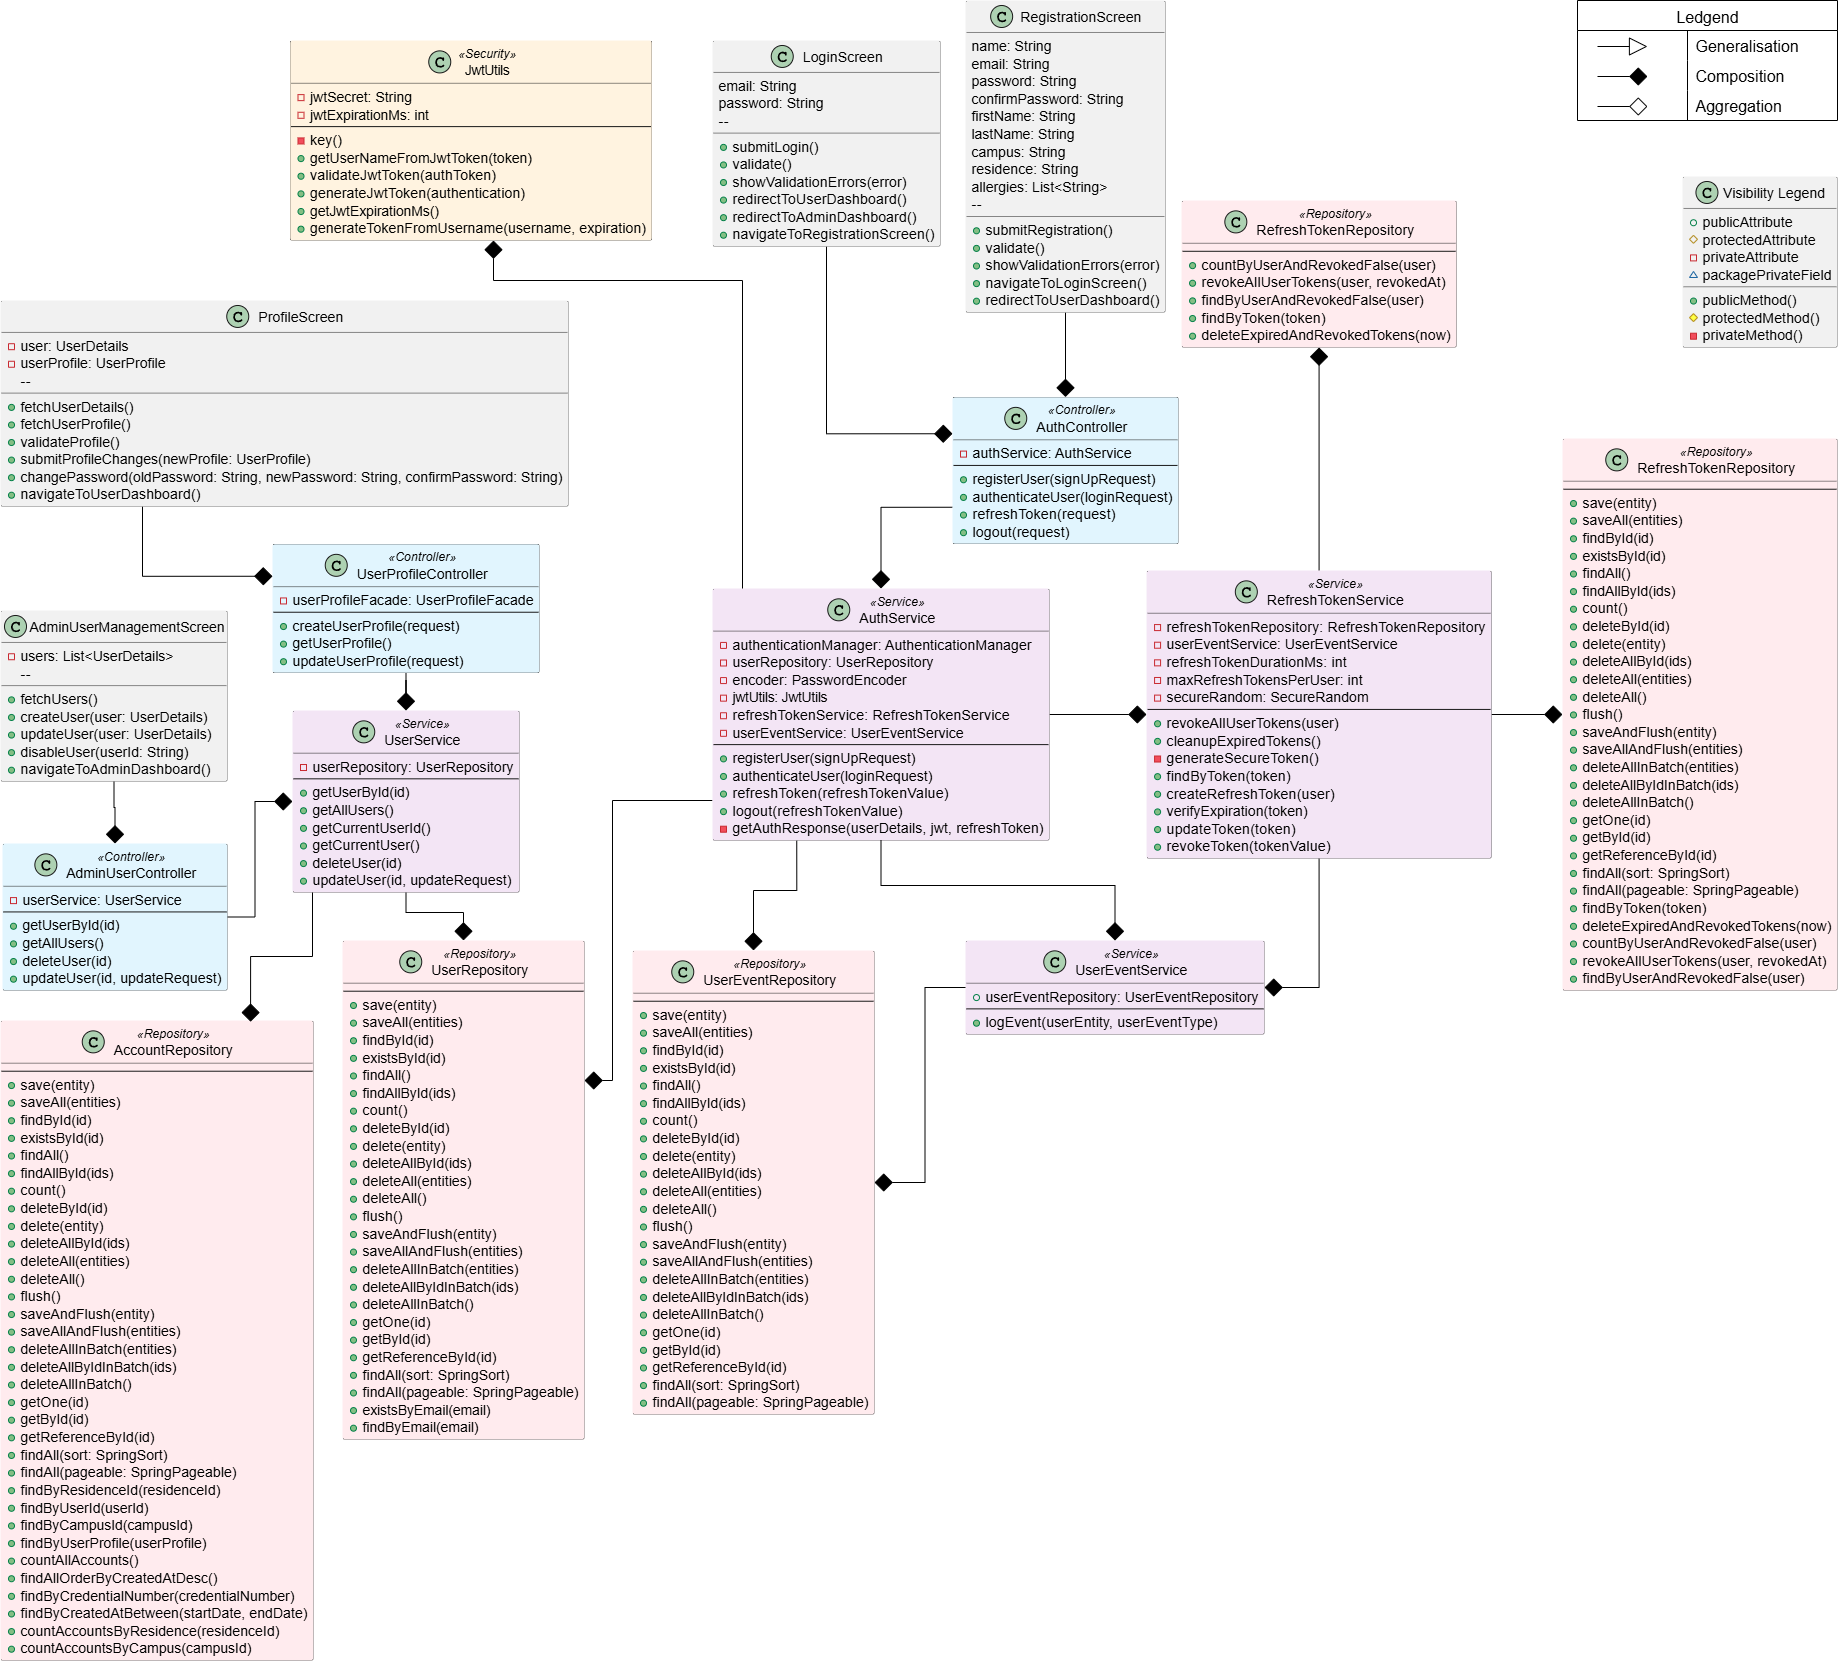
\includegraphics[width=\textwidth]{figures/class_diagrams/login-user-profile-subsystem.png}
    \caption{Gebruikerbestuur, intekening en registrasie klasdiagram}
    \label{fig:login_user_profile_class_diagram}
\end{figure}

Hier volg die CRC kaarte vir die belangrikste klasse in hierdie
onderdeel.

% JWTUtils beskrywing
\textbf{JWTUtils} is verantwoordelik vir die generering en validering van JWT tokens, wat gebruik word om gebruikers te verifieer en toegang tot die stelsel te beheer. Hierdie klas hanteer ook die koppeling van tokens aan spesifieke gebruikers.

\begin{table}[H]
\centering
\begin{tabular}{|p{0.4\textwidth}|p{0.4\textwidth}|}
    \hline
    \multicolumn{2}{|c|}{\textbf{JWTUtils}} \\
    \hline
    \textbf{Verantwoordelikhede} & \textbf{Medewerkers} \\
    \hline
    Genereer JWT token \newline
    Valideer JWT token \newline
    Vind die gebruiker wat die token besit \newline
    Genereer 'n JWT token vir 'n gebruiker
    & 
    JWT biblioteek \\
    \hline
\end{tabular}
\caption{CRC vir JWTUtils}
\label{tab:crc_jwt_utils}
\end{table}
\vspace{1em}

% LoginScreen beskrywing
\textbf{LoginScreen} verskaf die gebruikerskoppelvlak vir intekening. Dit neem die gebruiker se naam en wagwoord, valideer insette, en wys foutboodskappe indien nodig.

% CRC vir LoginScreen
\begin{table}[H]
\centering
\begin{tabular}{|p{0.4\textwidth}|p{0.4\textwidth}|}
    \hline
    \multicolumn{2}{|c|}{\textbf{LoginScreen}} \\
    \hline
    \textbf{Verantwoordelikhede} & \textbf{Medewerkers} \\
    \hline
    Verskaf gebruikersnaam en wagwoord vir intekening \newline
    Valideer insette \newline
    Wys foutboodskappe indien nodig
    &
    AuthController \\
    \hline
\end{tabular}
\caption{CRC vir LoginScreen}
\label{tab:crc_login_screen}
\end{table}
\vspace{1em}

% RegistrationScreen beskrywing
\textbf{RegistrationScreen} bied die koppelvlak vir nuwe gebruikers om te registreer. Dit versamel registrasie-inligting, valideer insette, en gee terugvoer oor sukses of foute.

% CRC vir RegistrationScreen
\begin{table}[H]
\centering
\begin{tabular}{|p{0.4\textwidth}|p{0.4\textwidth}|}
    \hline
    \multicolumn{2}{|c|}{\textbf{RegistrationScreen}} \\
    \hline
    \textbf{Verantwoordelikhede} & \textbf{Medewerkers} \\
    \hline
    Verskaf registrasie-inligting \newline
    Valideer insette \newline
    Wys sukses- of foutboodskappe
    &
    AuthController \\
    \hline
\end{tabular}
\caption{CRC vir RegistrationScreen}
\label{tab:crc_registration_screen}
\end{table}
\vspace{1em}

% AuthController beskrywing
\textbf{AuthController} hanteer alle intekening- en registrasieverwante versoeke vanaf die koppelvlak. Dit valideer gebruikersinligting en roep die dienslaag aan vir verdere verwerking.

% CRC vir AuthController
\begin{table}[H]
\centering
\begin{tabular}{|p{0.4\textwidth}|p{0.4\textwidth}|}
    \hline
    \multicolumn{2}{|c|}{\textbf{AuthController}} \\
    \hline
    \textbf{Verantwoordelikhede} & \textbf{Medewerkers} \\
    \hline
    Hanteer intekening en registrasie versoeke \newline
    Valideer gebruikersinligting \newline
    Roep dienslaag aan vir verifikasie en token generasie
    &
    AuthService \\
    \hline
\end{tabular}
\caption{CRC vir AuthController}
\label{tab:crc_auth_controller}
\end{table}
\vspace{1em}

% AuthService beskrywing
\textbf{AuthService} is die dienslaag wat verantwoordelik is vir die verifikasie van gebruikers, die generering en validering van tokens, en die hantering van sessies en verwante gebeurtenisse.

% CRC vir AuthService
\begin{table}[H]
\centering
\begin{tabular}{|p{0.4\textwidth}|p{0.4\textwidth}|}
    \hline
    \multicolumn{2}{|c|}{\textbf{AuthService}} \\
    \hline
    \textbf{Verantwoordelikhede} & \textbf{Medewerkers} \\
    \hline
    Verifieer gebruikersinligting \newline
    Genereer en valideer tokens \newline
    Hanteer sessies en gebeurtenisse
    &
    RefreshTokenService \newline
    UserEventService \newline
    JwtUtils \newline
    UserEventRepository \newline
    UserRepository  \newline
    RefreshTokenRepository  \\
    \hline
\end{tabular}
\caption{CRC vir AuthService}
\label{tab:crc_auth_service}
\end{table}
\vspace{1em}

% ProfileScreen beskrywing
\textbf{ProfileScreen} bied die koppelvlak waar gebruikers hul profiel kan besigtig en wysig. Dit valideer profielinligting en stuur veranderinge na die dienslaag.

% CRC vir ProfileScreen
\begin{table}[H]
\centering
\begin{tabular}{|p{0.4\textwidth}|p{0.4\textwidth}|}
    \hline
    \multicolumn{2}{|c|}{\textbf{ProfileScreen}} \\
    \hline
    \textbf{Verantwoordelikhede} & \textbf{Medewerkers} \\
    \hline
    Wys en wysig gebruikersprofiel \newline
    Valideer profielinligting \newline
    Stuur veranderinge na dienslaag
    &
    UserProfileController \\
    \hline
\end{tabular}
\caption{CRC vir ProfileScreen}
\label{tab:crc_profile_screen}
\end{table}
\vspace{1em}

% UserProfileController beskrywing
\textbf{UserProfileController} hanteer versoeke wat met gebruikersprofiele verband hou, en stuur gevalideerde data na die dienslaag vir verdere verwerking.

% CRC vir UserProfileController
\begin{table}[H]
\centering
\begin{tabular}{|p{0.4\textwidth}|p{0.4\textwidth}|}
    \hline
    \multicolumn{2}{|c|}{\textbf{UserProfileController}} \\
    \hline
    \textbf{Verantwoordelikhede} & \textbf{Medewerkers} \\
    \hline
    Hanteer profielversoeke \newline
    Valideer en stuur profieldata na dienslaag
    &
    UserService \\
    \hline
\end{tabular}
\caption{CRC vir UserProfileController}
\label{tab:crc_user_profile_controller}
\end{table}
\vspace{1em}

% UserService beskrywing
\textbf{UserService} verwerk alle gebruikersdata en hanteer logika wat met profiele en rekeninge verband hou.

% CRC vir UserService
\begin{table}[H]
\centering
\begin{tabular}{|p{0.4\textwidth}|p{0.4\textwidth}|}
    \hline
    \multicolumn{2}{|c|}{\textbf{UserService}} \\
    \hline
    \textbf{Verantwoordelikhede} & \textbf{Medewerkers} \\
    \hline
    Verwerk gebruikersdata \newline
    Hanteer profiel- en rekeningverwante logika
    &
    AccountRepository  \newline
    UserRepository \\
    \hline
\end{tabular}
\caption{CRC vir UserService}
\label{tab:crc_user_service}
\end{table}
\vspace{1em}

% AdminUserManagementScreen beskrywing
\textbf{AdminUserManagementScreen} is die administratiewe koppelvlak vir die bestuur van gebruikers. Administrateurs kan gebruikers besigtig, aktiveer, deaktiveer of verwyder.

% CRC vir AdminUserManagementScreen
\begin{table}[H]
\centering
\begin{tabular}{|p{0.4\textwidth}|p{0.4\textwidth}|}
    \hline
    \multicolumn{2}{|c|}{\textbf{AdminUserManagementScreen}} \\
    \hline
    \textbf{Verantwoordelikhede} & \textbf{Medewerkers} \\
    \hline
    Wys en bestuur gebruikerslys \newline
    Aktiveer, deaktiveer of verwyder gebruikers
    &
    AdminUserController \\
    \hline
\end{tabular}
\caption{CRC vir AdminUserManagementScreen}
\label{tab:crc_admin_user_management_screen}
\end{table}
\vspace{1em}

% AdminUserController beskrywing
\textbf{AdminUserController} hanteer administratiewe versoeke rakende gebruikersaksies en roep die dienslaag aan vir uitvoering van hierdie aksies.

% CRC vir AdminUserController
\begin{table}[H]
\centering
\begin{tabular}{|p{0.4\textwidth}|p{0.4\textwidth}|}
    \hline
    \multicolumn{2}{|c|}{\textbf{AdminUserController}} \\
    \hline
    \textbf{Verantwoordelikhede} & \textbf{Medewerkers} \\
    \hline
    Hanteer administratiewe gebruikersversoeke \newline
    Roep dienslaag aan vir
    gebruikersaksies &
    UserService \\
    \hline
\end{tabular}
\caption{CRC vir AdminUserController}
\label{tab:crc_admin_user_controller}
\end{table}
\vspace{1em}
